\section{Numerical comparison of the binning methods}

This section applies the preceding definitions to controlled synthetic samples. All samples contain $N=10^6$ observations and all random draws use a fixed seed so that the numerical comparison is reproducible. We compare the occupancy structure produced by \texttt{cut}, \texttt{qcut}, and logarithmic binning, then examine the empirical CCDFs and the conditional mean within each bin. The results show that no method dominates for every purpose: quantile bins control occupancy, equal-width bins preserve additive resolution, and logarithmic bins preserve multiplicative resolution while substantially improving representation of broad tails.

\subsection{Binning results for the three methods}

Table~\ref{tab:binning-results} reports a compact numerical diagnostic for $K=50$ bins. The minimum and maximum occupancies and the number of empty bins measure how unevenly each partition distributes observations. To summarize this unevenness with a dimensionless quantity, we use the coefficient of variation (CV) of the bin occupancies,
\begin{equation}
 \mathrm{CV}=\frac{s_n}{\bar n},
 \qquad
 \bar n=\frac{1}{K}\sum_{k=1}^{K}n_k=\frac{n}{K},
\end{equation}
where $s_n$ is the standard deviation of the $K$ bin counts and $\bar n$ is their mean. Thus $\mathrm{CV}=0$ corresponds to exactly equal occupancies, while larger values indicate increasingly concentrated bin counts.

\begin{table}[htbp]
\centering
\caption{Occupancy diagnostics for $N=10^6$ observations and $K=50$ bins. CV denotes the coefficient of variation of the bin counts.}
\label{tab:binning-results}
\renewcommand{\arraystretch}{1.22}
\begin{tabular*}{0.98\textwidth}{@{\extracolsep{\fill}}llcccc@{}}
\toprule
Distribution & Method & Min. count & Max. count & Empty bins & CV \\
\midrule
Exponential & cut & $0$ & $245{,}434$ & $5$ & $2.451$ \\
Exponential & qcut & $20{,}000$ & $20{,}000$ & $0$ & $0.000$ \\
Exponential & log binning & $0$ & $119{,}337$ & $1$ & $1.761$ \\
Lognormal & cut & $0$ & $214{,}121$ & $2$ & $2.458$ \\
Lognormal & qcut & $20{,}000$ & $20{,}000$ & $0$ & $0.000$ \\
Lognormal & log binning & $1$ & $76{,}481$ & $0$ & $1.304$ \\
Pareto & cut & $0$ & $999{,}874$ & $40$ & $6.999$ \\
Pareto & qcut & $20{,}000$ & $20{,}000$ & $0$ & $0.000$ \\
Pareto & log binning & $0$ & $258{,}976$ & $6$ & $2.538$ \\
\bottomrule
\end{tabular*}
\end{table}

The quantile result is exact here because $10^6$ is divisible by $50$ and the simulated samples are continuous, so ties at the quantile edges occur with probability zero. Every \texttt{qcut} bin contains $20{,}000$ observations. This property is useful when subsequent statistics should be estimated from groups with comparable sample sizes, although the corresponding widths can differ enormously.

The equal-width result exposes the heavy-tail problem. For the Pareto sample, $999{,}874$ of the $10^6$ observations fall into the most populated equal-width bin and $40$ of the $50$ bins are empty. The maximum observation determines such a large range that a linear partition becomes almost useless for resolving the body of the sample. In this particular run, the documented $0.1\%$ range extension used by \texttt{pandas.cut} when \texttt{bins} is an integer even moves the numerical lower edge below zero, despite every Pareto observation being positive; this is an edge-construction artifact caused by the enormous full range, not a property of the data. Logarithmic binning is far less concentrated because the widths expand geometrically, although its purpose is not to equalize counts and some far-tail bins remain empty in a finite sample. For the lognormal sample, logarithmic binning is particularly effective at avoiding empty intervals while retaining multiplicative resolution.

The ordinary histograms in Fig.~\ref{fig:synthetic-histograms} provide the complementary visual picture. As $K$ increases, the exponential and lognormal distributions acquire progressively finer resolution, whereas the Pareto distribution continues to require a representation adapted to its long tail.

\subsection{Complementary cumulative distributions}

Figure~\ref{fig:ccdf-grid} compares the empirical CCDF with an illustrative log--log ordinary least-squares fit for each of the three synthetic distributions. The three rows repeat the same CCDF for $K=25$, $50$, and $100$ only to preserve visual correspondence with the binning experiments; the CCDF itself is independent of $K$. This independence is one of its principal advantages, because the cumulative representation is constructed directly from the ordered sample rather than from histogram boundaries.

\begin{figure}[!htbp]
\centering
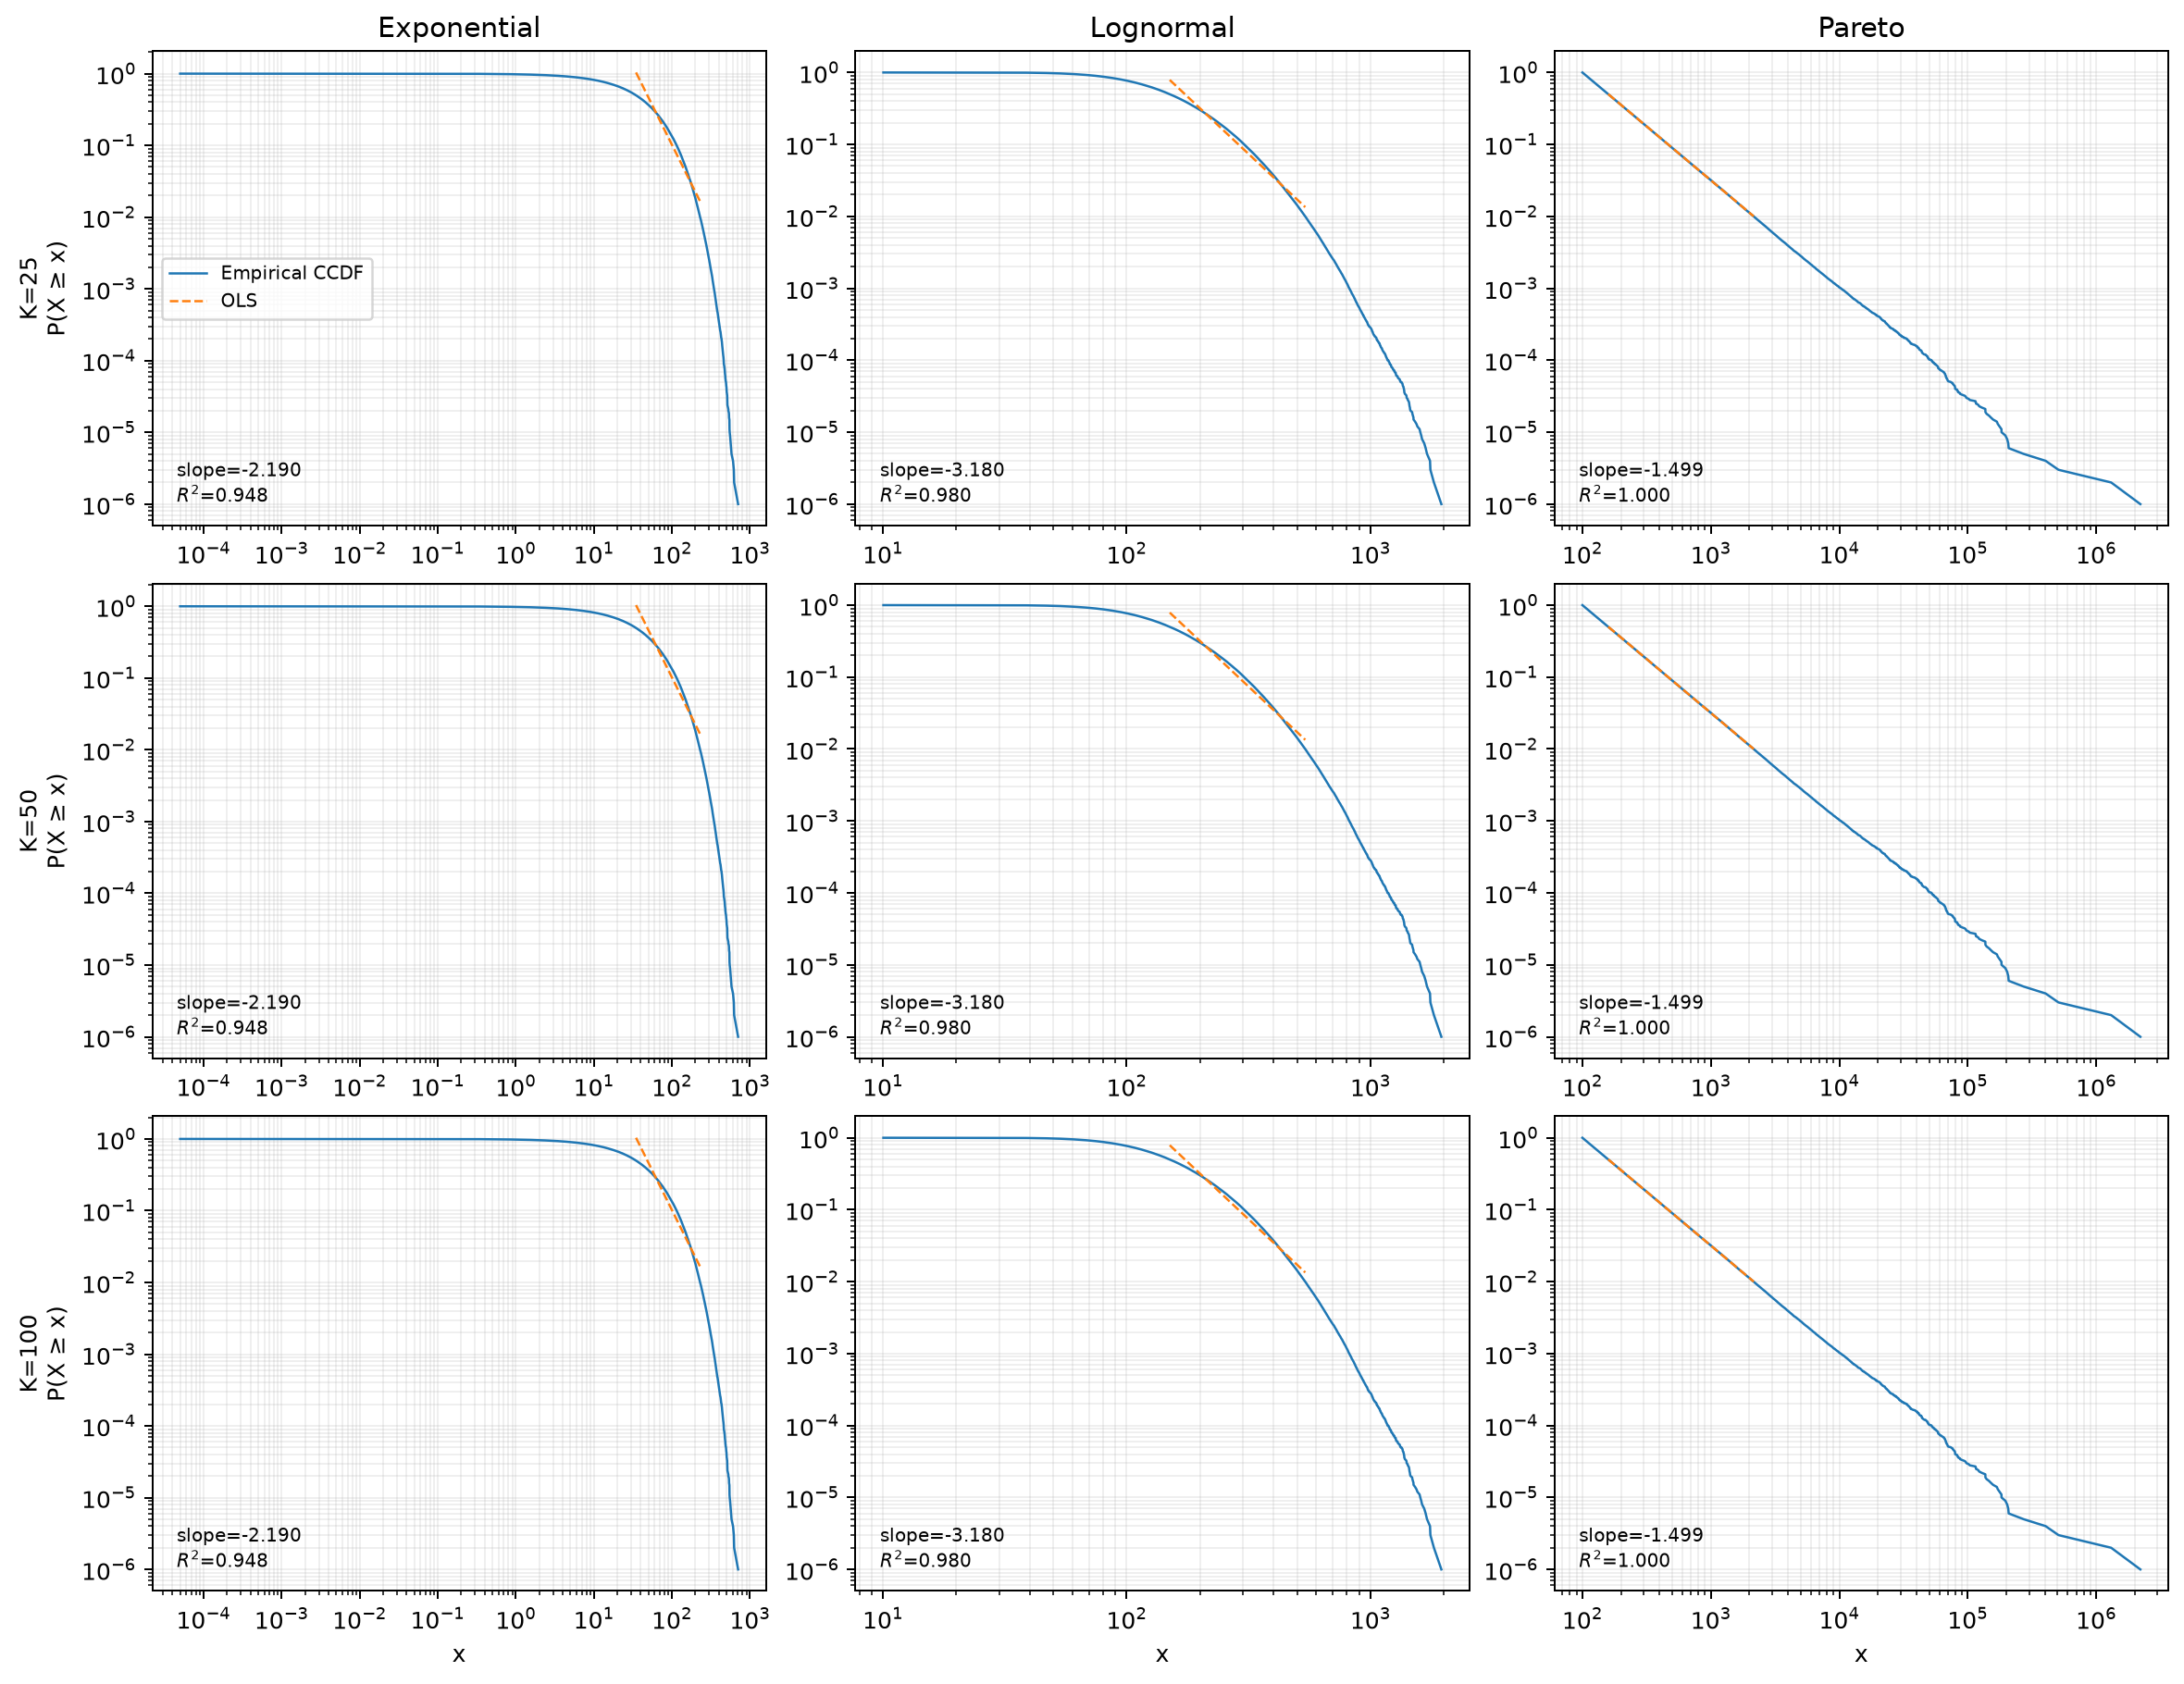
\includegraphics[width=0.92\textwidth]{assets/ccdf_grid_no_title.png}
\caption{Empirical complementary cumulative distributions for the exponential, lognormal, and Pareto samples. The repeated rows emphasize that the empirical CCDF is independent of the number of histogram bins. Dashed lines show an illustrative ordinary least-squares fit over a restricted survival-probability interval and should not be interpreted as a formal power-law test.}
\label{fig:ccdf-grid}
\end{figure}

For the exponential law,
\begin{equation}
 \overline F(x)=e^{-\lambda x},
\end{equation}
so a log--log plot is curved rather than linear. The lognormal CCDF is broad and may resemble a line over a limited interval, but it also develops systematic curvature. For the Pareto law in Eq.~\eqref{eq:pareto-ccdf},
\begin{equation}
 \log \overline F(x)
 =-(\alpha-1)\log x +(\alpha-1)\log x_{\min},
\end{equation}
which is exactly linear in log--log coordinates. With $\alpha=2.5$, the theoretical CCDF slope is $-1.5$.

The dashed ordinary least-squares lines in Fig.~\ref{fig:ccdf-grid} are included only as visual diagnostics. Clauset, Shalizi, and Newman \cite{ClausetShaliziNewman2009} show why least-squares regression on logarithmically transformed histograms or cumulative plots is generally inadequate for estimating and validating a power law. A proper empirical analysis should estimate the lower cutoff, fit the exponent by maximum likelihood, evaluate goodness of fit, and compare plausible alternative distributions.

\subsection{Mean value within each bin}

The mean of the observations assigned to a bin is a useful way to visualize what the partition does to the scale of the data. For bin $B_k$ with occupancy $n_k>0$, define
\begin{equation}
 \overline x_k
 =\frac{1}{n_k}\sum_{i:x_i\in B_k}x_i.
\end{equation}
Figure~\ref{fig:bin-means} plots this quantity against the bin index for the three methods, three distributions, and three values of $K$. The figure is the same reproducible asset generated by the numerical experiment pipeline; every panel contains its own legend so that the three binning methods remain identifiable without relying on another panel.

\begin{figure}[!htbp]
\centering
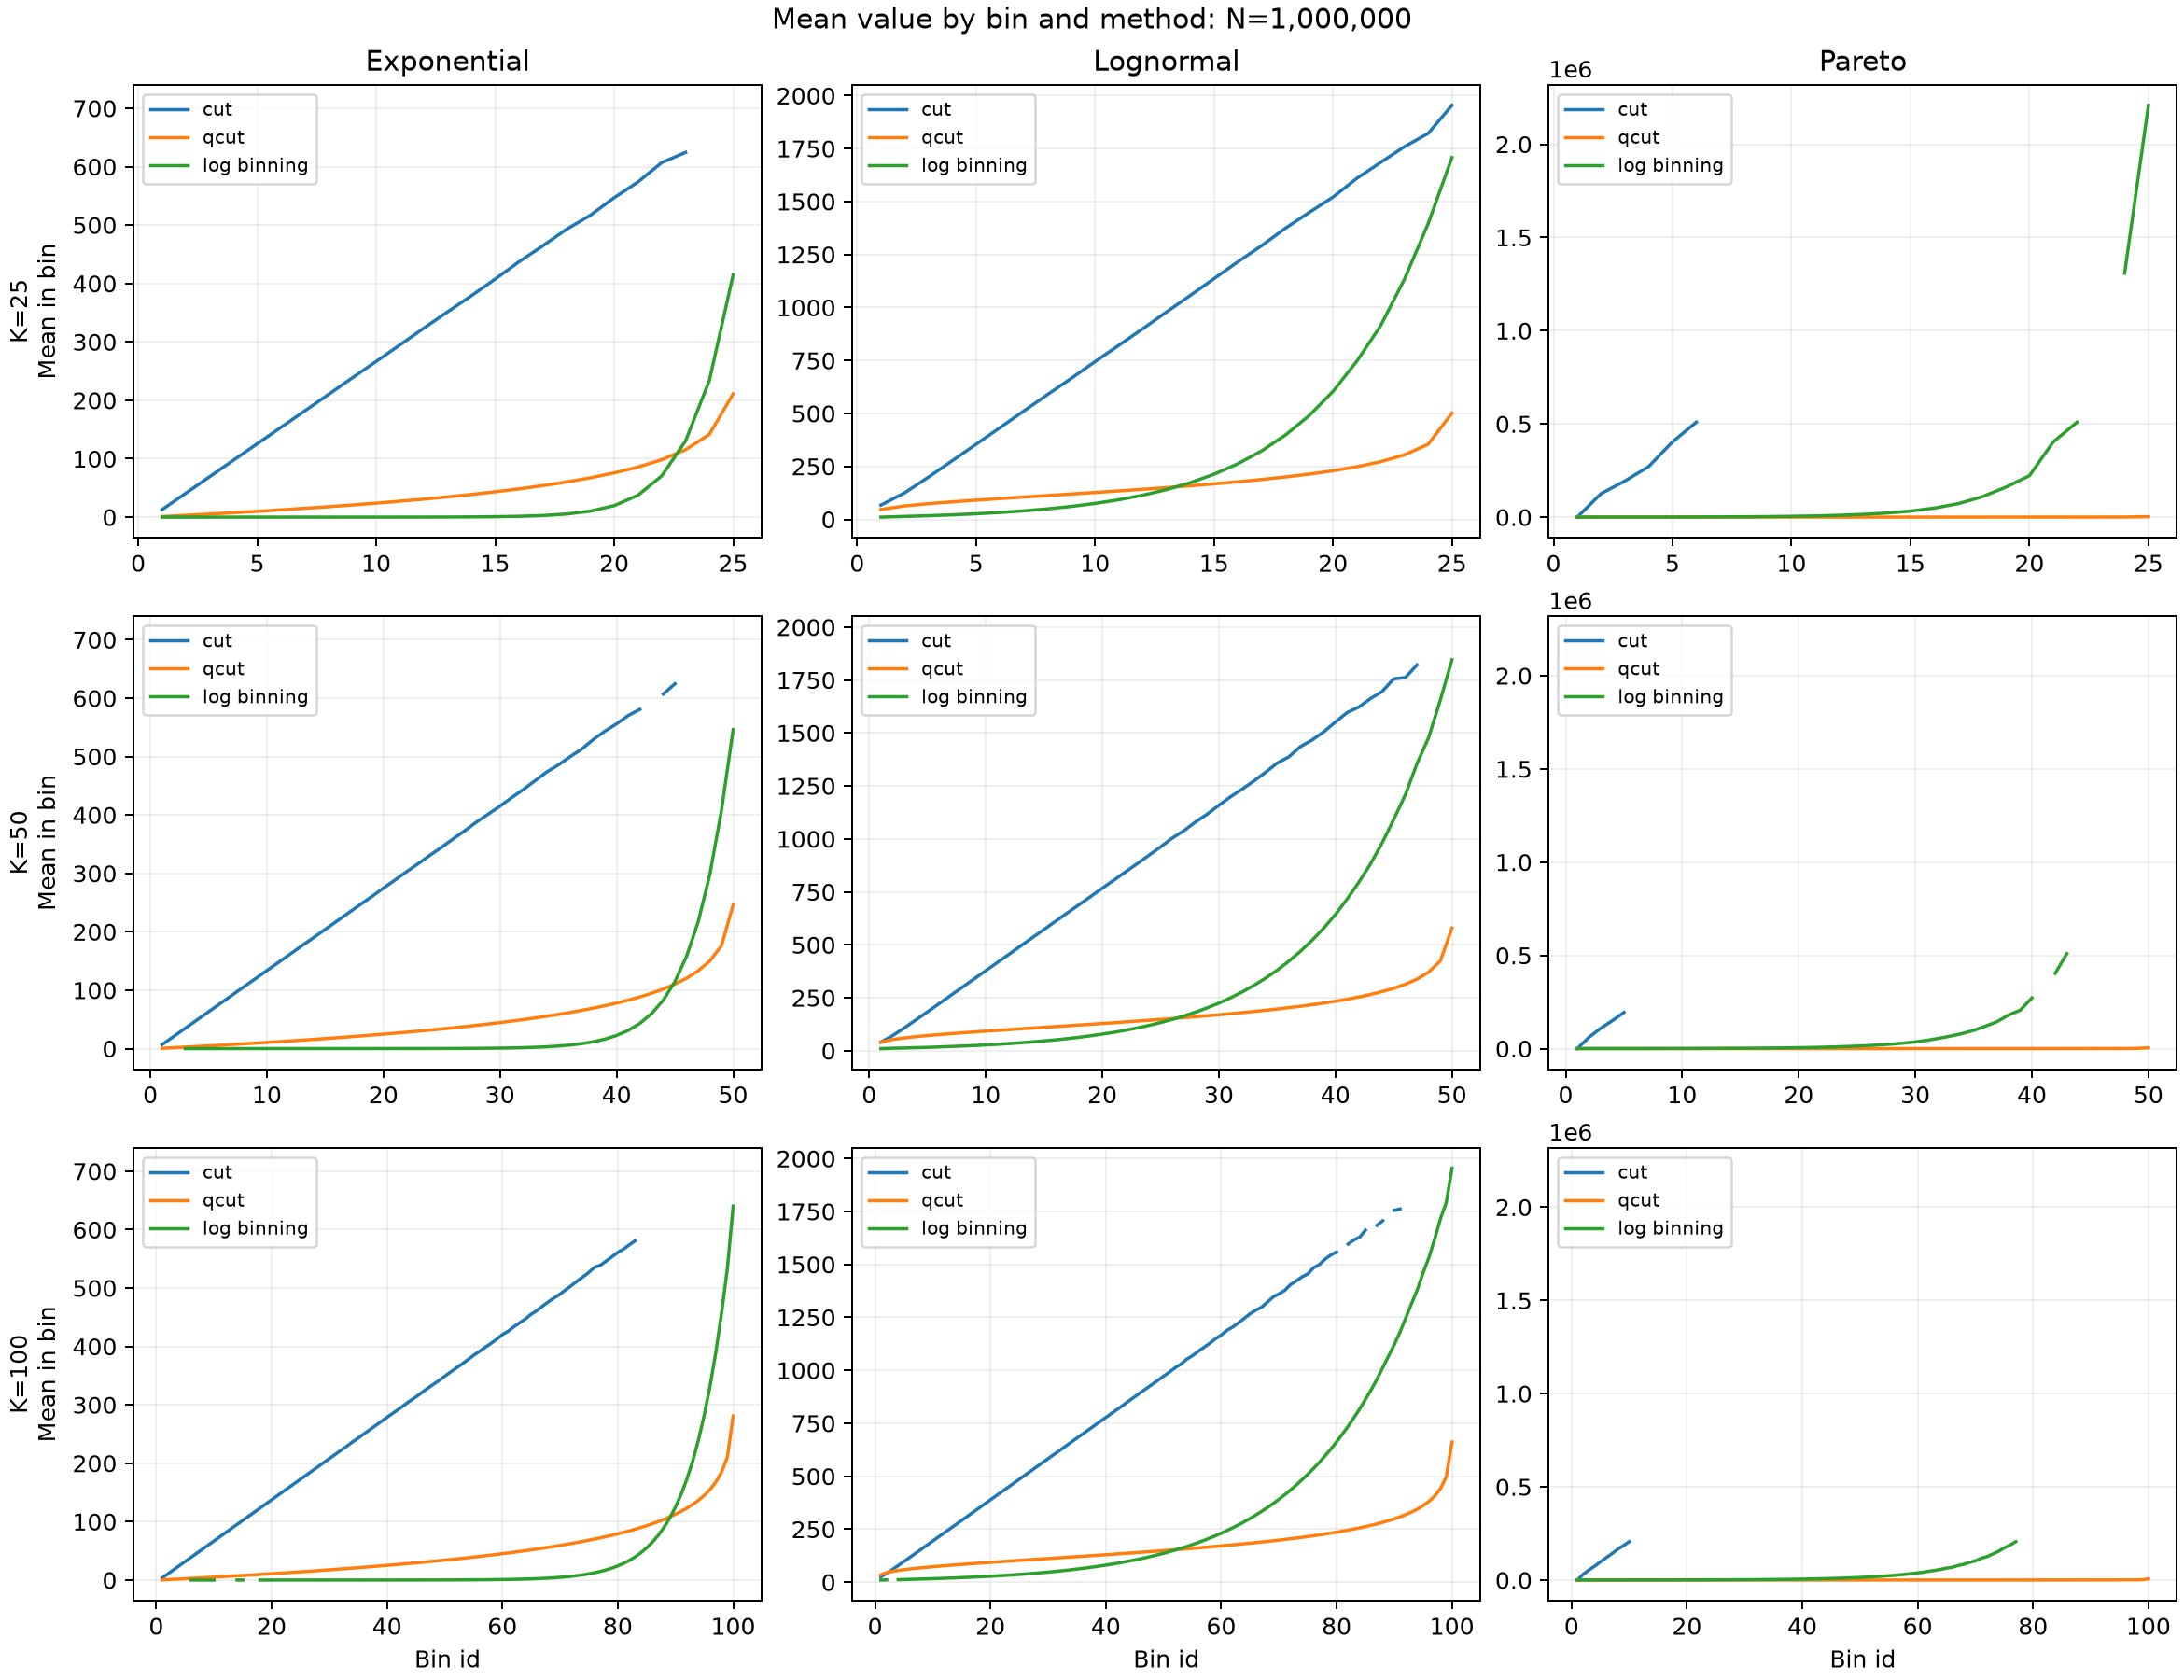
\includegraphics[width=0.92\textwidth]{bin_means_grid.png}
\caption{Mean observation within each bin for \texttt{cut}, \texttt{qcut}, and logarithmic binning. All nine panels use a linear vertical scale and contain their own legend.}
\label{fig:bin-means}
\end{figure}

The three curves have different interpretations because the index $k$ labels different geometries. Under \texttt{cut}, consecutive indices represent equal additive increments in $x$, so the mean of an occupied bin tends to track its interval center. Under \texttt{qcut}, consecutive indices represent equal increments of empirical probability, not equal increments of $x$. The upper quantile bins therefore become progressively wider for skewed data, and the final bin can have a mean much larger than the preceding bins. Under logarithmic binning, consecutive indices represent equal increments in $\log x$, so the characteristic scale of the bins grows geometrically.

The Pareto panels make the contrast most visible. The equal-width method produces a long sequence of sparse or empty high-index bins because a few extreme observations determine the total linear range. Quantile binning avoids empty groups by construction but places an increasingly broad interval into the upper quantiles. Logarithmic binning follows the multiplicative geometry of the tail and therefore distributes resolution more evenly across orders of magnitude. On a linear vertical axis, the extreme-bin means naturally dominate the Pareto panels; this is a genuine consequence of the long tail rather than a plotting defect.

Taken together, the results suggest a practical division of labor. Equal-width bins are appropriate when additive distances are the quantity of interest and the observed range is not dominated by extremes. Quantile bins are appropriate when comparable group sizes are required. Logarithmic bins are appropriate when positive data span several orders of magnitude and multiplicative resolution is more meaningful than additive resolution. The CCDF should be considered alongside all three because it retains the full ordering information without requiring any bin boundaries.
